% Options for packages loaded elsewhere
\PassOptionsToPackage{unicode}{hyperref}
\PassOptionsToPackage{hyphens}{url}
\PassOptionsToPackage{dvipsnames,svgnames,x11names}{xcolor}
%
\documentclass[
  letterpaper,
  DIV=11,
  numbers=noendperiod]{scrartcl}

\usepackage{amsmath,amssymb}
\usepackage{iftex}
\ifPDFTeX
  \usepackage[T1]{fontenc}
  \usepackage[utf8]{inputenc}
  \usepackage{textcomp} % provide euro and other symbols
\else % if luatex or xetex
  \usepackage{unicode-math}
  \defaultfontfeatures{Scale=MatchLowercase}
  \defaultfontfeatures[\rmfamily]{Ligatures=TeX,Scale=1}
\fi
\usepackage{lmodern}
\ifPDFTeX\else  
    % xetex/luatex font selection
\fi
% Use upquote if available, for straight quotes in verbatim environments
\IfFileExists{upquote.sty}{\usepackage{upquote}}{}
\IfFileExists{microtype.sty}{% use microtype if available
  \usepackage[]{microtype}
  \UseMicrotypeSet[protrusion]{basicmath} % disable protrusion for tt fonts
}{}
\makeatletter
\@ifundefined{KOMAClassName}{% if non-KOMA class
  \IfFileExists{parskip.sty}{%
    \usepackage{parskip}
  }{% else
    \setlength{\parindent}{0pt}
    \setlength{\parskip}{6pt plus 2pt minus 1pt}}
}{% if KOMA class
  \KOMAoptions{parskip=half}}
\makeatother
\usepackage{xcolor}
\setlength{\emergencystretch}{3em} % prevent overfull lines
\setcounter{secnumdepth}{-\maxdimen} % remove section numbering
% Make \paragraph and \subparagraph free-standing
\ifx\paragraph\undefined\else
  \let\oldparagraph\paragraph
  \renewcommand{\paragraph}[1]{\oldparagraph{#1}\mbox{}}
\fi
\ifx\subparagraph\undefined\else
  \let\oldsubparagraph\subparagraph
  \renewcommand{\subparagraph}[1]{\oldsubparagraph{#1}\mbox{}}
\fi


\providecommand{\tightlist}{%
  \setlength{\itemsep}{0pt}\setlength{\parskip}{0pt}}\usepackage{longtable,booktabs,array}
\usepackage{calc} % for calculating minipage widths
% Correct order of tables after \paragraph or \subparagraph
\usepackage{etoolbox}
\makeatletter
\patchcmd\longtable{\par}{\if@noskipsec\mbox{}\fi\par}{}{}
\makeatother
% Allow footnotes in longtable head/foot
\IfFileExists{footnotehyper.sty}{\usepackage{footnotehyper}}{\usepackage{footnote}}
\makesavenoteenv{longtable}
\usepackage{graphicx}
\makeatletter
\def\maxwidth{\ifdim\Gin@nat@width>\linewidth\linewidth\else\Gin@nat@width\fi}
\def\maxheight{\ifdim\Gin@nat@height>\textheight\textheight\else\Gin@nat@height\fi}
\makeatother
% Scale images if necessary, so that they will not overflow the page
% margins by default, and it is still possible to overwrite the defaults
% using explicit options in \includegraphics[width, height, ...]{}
\setkeys{Gin}{width=\maxwidth,height=\maxheight,keepaspectratio}
% Set default figure placement to htbp
\makeatletter
\def\fps@figure{htbp}
\makeatother
\newlength{\cslhangindent}
\setlength{\cslhangindent}{1.5em}
\newlength{\csllabelwidth}
\setlength{\csllabelwidth}{3em}
\newlength{\cslentryspacingunit} % times entry-spacing
\setlength{\cslentryspacingunit}{\parskip}
\newenvironment{CSLReferences}[2] % #1 hanging-ident, #2 entry spacing
 {% don't indent paragraphs
  \setlength{\parindent}{0pt}
  % turn on hanging indent if param 1 is 1
  \ifodd #1
  \let\oldpar\par
  \def\par{\hangindent=\cslhangindent\oldpar}
  \fi
  % set entry spacing
  \setlength{\parskip}{#2\cslentryspacingunit}
 }%
 {}
\usepackage{calc}
\newcommand{\CSLBlock}[1]{#1\hfill\break}
\newcommand{\CSLLeftMargin}[1]{\parbox[t]{\csllabelwidth}{#1}}
\newcommand{\CSLRightInline}[1]{\parbox[t]{\linewidth - \csllabelwidth}{#1}\break}
\newcommand{\CSLIndent}[1]{\hspace{\cslhangindent}#1}

\KOMAoption{captions}{tablesignature}
\makeatletter
\@ifpackageloaded{tcolorbox}{}{\usepackage[skins,breakable]{tcolorbox}}
\@ifpackageloaded{fontawesome5}{}{\usepackage{fontawesome5}}
\definecolor{quarto-callout-color}{HTML}{909090}
\definecolor{quarto-callout-note-color}{HTML}{0758E5}
\definecolor{quarto-callout-important-color}{HTML}{CC1914}
\definecolor{quarto-callout-warning-color}{HTML}{EB9113}
\definecolor{quarto-callout-tip-color}{HTML}{00A047}
\definecolor{quarto-callout-caution-color}{HTML}{FC5300}
\definecolor{quarto-callout-color-frame}{HTML}{acacac}
\definecolor{quarto-callout-note-color-frame}{HTML}{4582ec}
\definecolor{quarto-callout-important-color-frame}{HTML}{d9534f}
\definecolor{quarto-callout-warning-color-frame}{HTML}{f0ad4e}
\definecolor{quarto-callout-tip-color-frame}{HTML}{02b875}
\definecolor{quarto-callout-caution-color-frame}{HTML}{fd7e14}
\makeatother
\makeatletter
\makeatother
\makeatletter
\makeatother
\makeatletter
\@ifpackageloaded{caption}{}{\usepackage{caption}}
\AtBeginDocument{%
\ifdefined\contentsname
  \renewcommand*\contentsname{Table of contents}
\else
  \newcommand\contentsname{Table of contents}
\fi
\ifdefined\listfigurename
  \renewcommand*\listfigurename{List of Figures}
\else
  \newcommand\listfigurename{List of Figures}
\fi
\ifdefined\listtablename
  \renewcommand*\listtablename{List of Tables}
\else
  \newcommand\listtablename{List of Tables}
\fi
\ifdefined\figurename
  \renewcommand*\figurename{Figure}
\else
  \newcommand\figurename{Figure}
\fi
\ifdefined\tablename
  \renewcommand*\tablename{Table}
\else
  \newcommand\tablename{Table}
\fi
}
\@ifpackageloaded{float}{}{\usepackage{float}}
\floatstyle{ruled}
\@ifundefined{c@chapter}{\newfloat{codelisting}{h}{lop}}{\newfloat{codelisting}{h}{lop}[chapter]}
\floatname{codelisting}{Listing}
\newcommand*\listoflistings{\listof{codelisting}{List of Listings}}
\makeatother
\makeatletter
\@ifpackageloaded{caption}{}{\usepackage{caption}}
\@ifpackageloaded{subcaption}{}{\usepackage{subcaption}}
\makeatother
\makeatletter
\@ifpackageloaded{tcolorbox}{}{\usepackage[skins,breakable]{tcolorbox}}
\makeatother
\makeatletter
\@ifundefined{shadecolor}{\definecolor{shadecolor}{rgb}{.97, .97, .97}}
\makeatother
\makeatletter
\makeatother
\makeatletter
\makeatother
\ifLuaTeX
  \usepackage{selnolig}  % disable illegal ligatures
\fi
\IfFileExists{bookmark.sty}{\usepackage{bookmark}}{\usepackage{hyperref}}
\IfFileExists{xurl.sty}{\usepackage{xurl}}{} % add URL line breaks if available
\urlstyle{same} % disable monospaced font for URLs
\hypersetup{
  pdftitle={What They Forgot to Tell You About Machine Learning with an Application to Pharmaceutical Manufacturing},
  pdfauthor={Kjell Johnson; Max Kuhn},
  colorlinks=true,
  linkcolor={blue},
  filecolor={Maroon},
  citecolor={Blue},
  urlcolor={Blue},
  pdfcreator={LaTeX via pandoc}}

\title{What They Forgot to Tell You About Machine Learning with an
Application to Pharmaceutical Manufacturing}
\author{Kjell Johnson \and Max Kuhn}
\date{}

\begin{document}
\maketitle
\begin{abstract}
Predictive models (a.k.a. machine learning models) are ubiquitous in all
stages of drug research, safety, development, manufacturing, and
marketing. The results of these models are used inside and outside of
pharmaceutical companies for the purpose of understanding scientific
processes and for predicting characteristics of new samples or patients.
While there are many resources that describe such models, there are few
that explain how to develop a robust model that extracts the highest
possible performance from the available data, especially in support of
pharmaceutical applications. This tutorial will describe pitfalls and
best practices for developing and validating predictive models with a
specific application to a monitoring a pharmaceutical manufacturing
process. The pitfalls and best practices will be highlighted to call
attention to specific points that are not generally discussed in other
resources.
\end{abstract}
\ifdefined\Shaded\renewenvironment{Shaded}{\begin{tcolorbox}[interior hidden, frame hidden, borderline west={3pt}{0pt}{shadecolor}, breakable, sharp corners, boxrule=0pt, enhanced]}{\end{tcolorbox}}\fi

\hypertarget{introduction}{%
\section{Introduction}\label{introduction}}

It feels like machine learning (ML) is everywhere. Even after years of
popularity, tools such as ChatGPT\footnote{\href{https://chat.openai.com/}{\texttt{https://chat.openai.com}}}
have increased the visibility of ML and artificial intelligence even
further. These tools initially showed their use in image recognition
(``Is there a cat in this picture?'') and natural language processing
(e.g., grammar correction sentence completion). New tools can often take
a textual prompt and, with varying levels of success, complete some
tasks. Models can be used to rewrite an author's biography in iambic
pentameter, write program code, or describe the results of a
visualization.

In terms of data analysis used in drug R\&D, machine learning has been
in a statistician's toolbox for some time. It has been used for making
predictions during compound optimization, target discovery, in silico
modeling of absorption, distribution, metabolism, excretion, and
toxicology (ADMET) endpoints, etc.

This tutorial assumes that the reader has had some exposure to machine
learning (a.k.a. predictive modeling or statistical learning) and
related techniques such as resampling. If not, we suggest Hastie,
Tibshirani, and Friedman (2017) for technical information and Kuhn and
Johnson (2013) for practical descriptions focused on applying these
methods. For deep learning methods, Goodfellow, Bengio, and Courville
(2016) and Charu (2018) are good introductions.

Our goal is to discuss more realistic approaches to using machine
learning in preclinical applications, specifically Chemistry,
Manufacturing, and Control (CMC) applications. The structure takes a
relatively ordinary experimental problem (predicting drug concentration
using spectroscopy) to frame a discussion about what machine learning
can, can't do, and probably should do. The idea is that most machine
learning training materials are not holistic examinations of how the
process actually works. While describing our analysis, we will highlight
``what they forgot to tell you'' about these tools.

For example, it might make sense to discuss what the term ``machine
learning'' means and under what circumstances it is appropriate.
Historically, it usually connotes a specific type of black-block model,
such as a neural network or support vector machine. This leads us to our
first \emph{what they forgot} (WTF):

\begin{tcolorbox}[enhanced jigsaw, title=\textcolor{quarto-callout-important-color}{\faExclamation}\hspace{0.5em}{\textbf{WTF} \#1}, rightrule=.15mm, leftrule=.75mm, bottomtitle=1mm, opacityback=0, opacitybacktitle=0.6, bottomrule=.15mm, arc=.35mm, colframe=quarto-callout-important-color-frame, breakable, toprule=.15mm, toptitle=1mm, colback=white, titlerule=0mm, coltitle=black, left=2mm, colbacktitle=quarto-callout-important-color!10!white]

Whether a model is a ``machine learning model'' depends on how it will
be used rather than the mathematical definition of the technique. If the
goal of an analysis is to make the most accurate prediction possible,
it's fair to use the ML label.

\end{tcolorbox}

It is difficult to argue that ML models focus on making the most
accurate prediction of a new sample based on historical data. From that
point of view, any sufficiently complex model that performs sufficiently
well. For example, a linear regression model could fit this definition
by including appropriate interactions or nonlinear terms, such as spline
basis expansions. The models most representative of the current
zeitgeist are sophisticated and impenetrable methods such as neural
networks and boosted trees. However\ldots{}

\begin{tcolorbox}[enhanced jigsaw, title=\textcolor{quarto-callout-important-color}{\faExclamation}\hspace{0.5em}{\textbf{WTF} \#2}, rightrule=.15mm, leftrule=.75mm, bottomtitle=1mm, opacityback=0, opacitybacktitle=0.6, bottomrule=.15mm, arc=.35mm, colframe=quarto-callout-important-color-frame, breakable, toprule=.15mm, toptitle=1mm, colback=white, titlerule=0mm, coltitle=black, left=2mm, colbacktitle=quarto-callout-important-color!10!white]

You probably don't need a complex black-box machine learning model
(e.g.~deep neural networks, large ensemble models, etc.).

\end{tcolorbox}

Why not? First, not all problems are purely prediction problems. Most
black-box models used for ML are excellent at prediction but poor at
almost anything else. We have seen applications where simple two-factor
experimental data were analyzed using the random forest ensemble method
instead of a simple two-way ANOVA model. When it comes to judging what
predictors are important to the outcome(s), many machine learning models
are probably not applicable.

Another reason is the potential limitations of experimental data.
Sometimes, there is not enough data to support fitting such a model. For
example, if an unreplicated response surface design were available,
training a model and characterizing its efficacy with so few data points
would be difficult. Data size is a limitation, but there are other
challenging data characteristics: irrelevant predictors, measurement
system noise, censored values, multicollinearity, and others.

For some, there is a significant urge to fit complex ML models since
they often are the best choice in completely different domains, such as
the image analysis or generative prompt examples given previously. These
domains often have access to excessive amounts of non-tabular data.
These are data structures that do not naturally fit into the traditional
rectangular data format (e.g., spreadsheets or database tables). These
models are often complex deep-learning neural networks.

A disconnect occurs because most experimental data used in CMC
applications are tabular (or can be made to be tabular).

\begin{tcolorbox}[enhanced jigsaw, title=\textcolor{quarto-callout-important-color}{\faExclamation}\hspace{0.5em}{\textbf{WTF} \#3}, rightrule=.15mm, leftrule=.75mm, bottomtitle=1mm, opacityback=0, opacitybacktitle=0.6, bottomrule=.15mm, arc=.35mm, colframe=quarto-callout-important-color-frame, breakable, toprule=.15mm, toptitle=1mm, colback=white, titlerule=0mm, coltitle=black, left=2mm, colbacktitle=quarto-callout-important-color!10!white]

Unless you are analyzing a large number of images, it is exceedingly
unlikely that a deep-learning model is your best option.

\end{tcolorbox}

There is considerable anecdotal evidence that highly complex neural
networks may not perform well for reasonably sized tabular data sets.
This is currently being examined more formally in the literature (Kadra
et al. 2021; Gorishniy et al. 2021; Borisov et al. 2022; Shwartz-Ziv and
Armon 2022). Experimental data in preclinical applications can often
exhibit multicollinearity between predictors and data measured with
error. For novel data sets, we often do not know which predictors have a
relationship with the outcome, increasing the possibility that some
irrelevant predictors will be used to fit the model. In general, neural
networks do not thrive in these environments (Kuhn and Johnson 2013).

Simply put, deep learning models can be effective in specific scenarios
but are inappropriate in many other situations.

In this tutorial, we will discuss the process of constructing ML models
for a specific tabular data set. This process starts with understanding
the available data's predictors and responses. After this initial
understanding, we must then determine how to spend the data for the
model-building process. Specifically, some data will need to be used to
learn the generalizable characteristics that relate the predictors with
the response (i.e., the training set). And other data will need to be
used to assess how well the model predicts new data (i.e., the test
set). After splitting the data, the predictors and/or the response may
need to be pre-processed prior to modeling to enable models to better
extract the predictive signal. The next step is to select the types of
models which will be trained on the data. Each model has one or more
parameters that determine how predictors are related to the response. In
general, we do not know a priori which values of the tuning parameters
are best. Therefore, a process must be implemented that searches for an
optimal parameter set. After identifying an optimal model, this model is
then evaluated on the test data to determine if the model can be trusted
to predict new yet-to-be-seen samples reliably.

Let's look at a specific CMC application to facilitate the discussion
further.

\hypertarget{experimental-setting}{%
\section{Experimental setting}\label{experimental-setting}}

The manufacturing process of a biological drug is complex and requires
careful monitoring to ensure that the cells are efficiently creating the
drug product. This process can be very challenging to systematically
control since the incubation process can take many days, and cells are
complex biological entities that are affected by slight changes in
environmental conditions. To ensure that the bioreactor conditions are
conducive to the cells producing product, key attributes are measured by
sampling the contents of the bioreactor daily. If attributes are not in
an acceptable range, then steps must be taken to alter the conditions of
the bioreactor. Generally, the sooner the conditions can be adjusted,
the better the quantity and quality of the final drug product. Measuring
the attributes takes time. Therefore, there is usually a lag between the
attribute measurements and the corresponding adjustment. This lag can
lead to less and lower-quality products.

Raman spectroscopy is a tool that can measure chemical characteristics
(i.e., a chemical fingerprint) of samples in real-time (Jesus,
Löbenberg, and Bou-Chacra 2020; Esmonde-White, Cuellar, and Lewis 2022;
Silge et al. 2022). Using the spectra in a predictive model of the
characteristics of interest would enable real-time knowledge of and
corresponding adjustments to the bioreactor, thus generating higher
quality, larger volume drug product.

In the example outlined in this tutorial, several key input parameters
were varied systematically across their operating ranges within each of
the 60 small-scale bioreactors for producing a biological drug. Seven
days after the start of the experiment, a sample was collected and
analyzed by Raman spectroscopy. The concentration of the drug product in
the sample was also measured. This analysis aims to understand how
predictive Raman spectra can be of the drug product concentration. If
there is a relationship, then the model could be used to signal if the
bioreactor was insufficiently producing a product and prompting remedial
steps to increase production.

\hypertarget{sec-understanding-the-data}{%
\section{Understanding the Data}\label{sec-understanding-the-data}}

The first step in any modeling process is to understand the available
data.

\begin{tcolorbox}[enhanced jigsaw, title=\textcolor{quarto-callout-important-color}{\faExclamation}\hspace{0.5em}{\textbf{WTF} \#4}, rightrule=.15mm, leftrule=.75mm, bottomtitle=1mm, opacityback=0, opacitybacktitle=0.6, bottomrule=.15mm, arc=.35mm, colframe=quarto-callout-important-color-frame, breakable, toprule=.15mm, toptitle=1mm, colback=white, titlerule=0mm, coltitle=black, left=2mm, colbacktitle=quarto-callout-important-color!10!white]

The only way to be comfortable with your data is to never look at them.

\end{tcolorbox}

In this application, there is one sample from each of the 60
bioreactors. Raman spectroscopy has been applied to each sample, and the
drug product concentration has been measured.
Figure~\ref{fig-raman-spectra} displays the original Raman spectra. From
this figure, we can see that there is an initial downward trend towards
the middle of the wavenumbers, then an upward trend towards the higher
wavenumbers. The intensities are not randomly scattered. Instead, there
is a relationship across wavenumbers with intensity. This relationship
indicates that wavenumber intensities are correlated with each other. In
fact, the correlation between the majority of adjacent wavenumbers is
greater than 0.99.

\begin{figure}[t!]

{\centering \includegraphics[width=0.8\textwidth,height=\textheight]{figures/fig-raman-spectra-1.pdf}

}

\caption{\label{fig-raman-spectra}Raman spectra profiles for each of the
60 samples.}

\end{figure}

To illustrate this more clearly, let's examine the relationship among
wavenumber measurements for the first sample. To do this we will create
lags of the wavelength measurements. To create a lag, the data is
shifted by a specified number of rows to create a new variable. For
example, to create the first lag, the wavenumber measurements are
shifted over by one wavenumber. To create the second lag, the
measurements are shifted by two wavenumbers, and so on.
Figure~\ref{fig-lagged-spectra} illustrates the correlation between each
subsequent lag for the first 1000 lags. Clearly, close wavenumbers have
a high correlation, whereas far wavenumbers have a low correlation. As
we will see, understanding this characteristic will be very important
when deciding how to pre-process the data prior to modeling and which
models to train.

\begin{figure}[t!]

{\centering 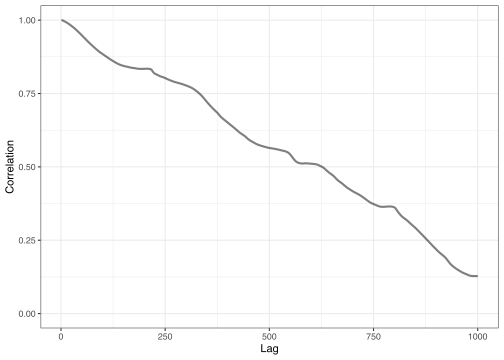
\includegraphics[width=0.8\textwidth,height=\textheight]{figures/fig-lagged-spectra-1.pdf}

}

\caption{\label{fig-lagged-spectra}The correlation between the original
intensities and lagged intensities for the first sample. As wavenumbers
depart, the correlation of the intensities decreases.}

\end{figure}

With such a large dimensional data set, it is difficult to investigate
specific predictors visually. Additionally, the high degree of
between-predictor correlations further decreases the ability to
investigate the data. In the pre-processing section, we'll look at
specific data points using dimension reduction tools under different
types of signal processing regimes.

In addition to understanding the predictors, we should also understand
the characteristics of the response. Examining the response distribution
can help determine if a transformation may be necessary or detect
unusual outcome values. Figure~\ref{fig-concentration} presents the
histogram of drug product concentration across the samples. For this
data, the distribution is approximately symmetric and has a range of 85
to 115. Based on this figure, a transformation does not appear
necessary, and there are no unusual samples.

\begin{figure}[t!]

{\centering 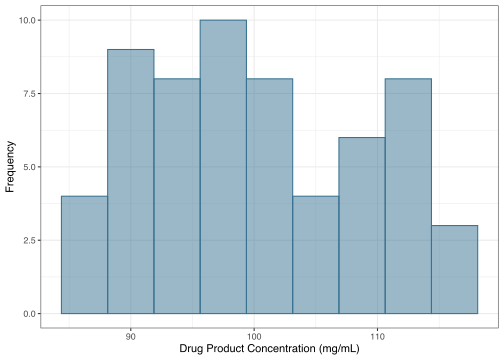
\includegraphics[width=0.6\textwidth,height=\textheight]{figures/fig-concentration-1.pdf}

}

\caption{\label{fig-concentration}The distribution of drug product
concentration across samples.}

\end{figure}

\hypertarget{data-spending}{%
\section{Data Spending}\label{data-spending}}

The primary objective of predictive modeling is to use the existing data
to develop a model that predicts new samples as accurately as possible.
To achieve this objective, a process must be implemented that avoids
over-fitting to the existing data (Kuhn and Johnson 2013; Hawkins 2004).
An over-fit model is one that accurately predicts the response for the
data on which the model was trained but does not accurately predict new
data. To avoid over-fitting, we must construct a model-building process
that mimics the prediction process for new samples. One way to do this
would be to split the data into training and test sets. A model could be
constructed with the training set, then predictive performance could be
evaluated with the test set.

\begin{tcolorbox}[enhanced jigsaw, title=\textcolor{quarto-callout-important-color}{\faExclamation}\hspace{0.5em}{\textbf{WTF} \#5}, rightrule=.15mm, leftrule=.75mm, bottomtitle=1mm, opacityback=0, opacitybacktitle=0.6, bottomrule=.15mm, arc=.35mm, colframe=quarto-callout-important-color-frame, breakable, toprule=.15mm, toptitle=1mm, colback=white, titlerule=0mm, coltitle=black, left=2mm, colbacktitle=quarto-callout-important-color!10!white]

Always have an independent data set that can contradict what you think
you may know.

\end{tcolorbox}

However, most predictive models must be constructed using a variety of
tuning parameter values. The test set would then need to be evaluated
multiple times to assess predictive performance. When the test set is
evaluated multiple times, we are essentially finding a model that fits
the test set. This process leads to over-fitting, and the model
performance cannot be trusted to evaluate the predictive performance on
new samples accurately. Therefore, a single training/test split will not
be adequate for building predictive models. Moreover, it is important to
understand that the test set should only be used once to evaluate the
final selected models.

Instead of a single training/test split, we need a process that can be
used to evaluate many tuning parameter values for each of many different
models. Figure~\ref{fig-resampling} illustrates a two-layered process
that incorporates the use of resampling. The first layer splits the
entire data set into a training and test set. In general, anywhere
between 50\% to 80\% of the data is randomly selected for the training
data, while the remaining data is placed in the test set. A random split
may be adequate but, in some cases, we can use \emph{stratified}
splitting. This can help keep the distribution of some variables
relatively the same between the training and testing sets.

\begin{figure}[t!]

{\centering \includegraphics[width=0.8\textwidth,height=\textheight]{premade/resampling.pdf}

}

\caption{\label{fig-resampling}Illustration of a general data usage
scheme that incorporates resampling.}

\end{figure}

The training data is further split into resamples as shown in the second
layer of Figure~\ref{fig-resampling}. Resampling methods make alternate
versions of the training set via additional partitions. Cross-validation
is one of the more popular resampling schemes. It could be used in this
layer, where the data is split into \(V\) folds. For example, if 10-fold
cross-validation were used in this layer, then the training data would
be partitioned into 10 folds. The analysis set for the first resample
would contain 9 folds of the data, while the assessment set would
contain 1 fold of the data. A model would be constructed using the 9
folds and would evaluated using the hold-out fold. To create the
analysis set for the second resample, a different combination of 9-folds
would be used to construct the model. The model would then be evaluated
on the fold that was not used in the modeling. For illustration,
Figure~\ref{fig-three-fold} provides an illustration of 3-fold
cross-validation (although \(V = 10\) is a much better choice).

\begin{tcolorbox}[enhanced jigsaw, title=\textcolor{quarto-callout-important-color}{\faExclamation}\hspace{0.5em}{\textbf{WTF} \#6}, rightrule=.15mm, leftrule=.75mm, bottomtitle=1mm, opacityback=0, opacitybacktitle=0.6, bottomrule=.15mm, arc=.35mm, colframe=quarto-callout-important-color-frame, breakable, toprule=.15mm, toptitle=1mm, colback=white, titlerule=0mm, coltitle=black, left=2mm, colbacktitle=quarto-callout-important-color!10!white]

Creating a test set does not prevent model overfitting when used
improperly. We have seen many examples where a practitioner will use
cross-validation to select optimal tuning parameters, then assess the
performance on the test set. This process is then repeated until
acceptable test set performance is found. The test set is no longer an
independent set for assessing model performance.

\end{tcolorbox}

\begin{figure}[t!]

{\centering 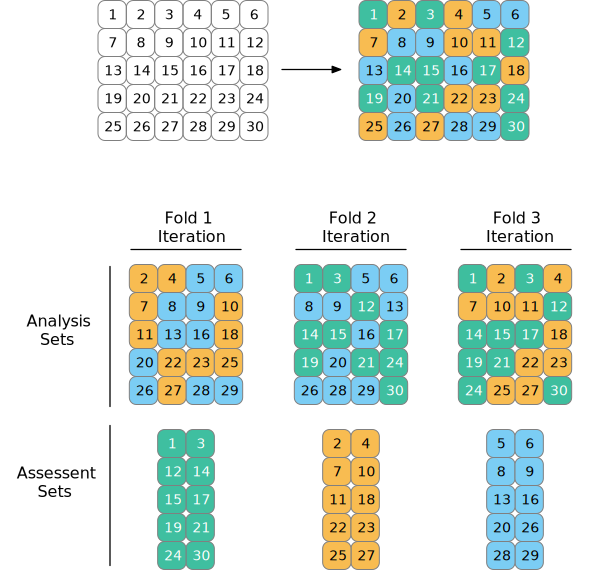
\includegraphics[width=0.6\textwidth,height=\textheight]{premade/three-CV.pdf}

}

\caption{\label{fig-three-fold}A diagram of how 3-fold cross-validation
can be used with 30 data points.}

\end{figure}

For the example presented here, a stratified random approach will be
used to split the data into a training (75\%) and a test (25\%) set. The
distribution of the response will be used as the stratification variable
such that an equal proportion of samples will be randomly selected
within each quartile of the distribution.

\hypertarget{sec-pre-processing}{%
\section{Pre-processing}\label{sec-pre-processing}}

The raw predictor and response data may not in the best form to allow
models reach their full predictive potential. The original data may
contain highly correlated predictors, predictors that lack information,
missing values, multi-category predictors, or highly skewed predictors.
Some models, such as those based on recursive partitioning algorithms,
can handle most of these challenging characteristics. However, many
models either cannot be built, or the predictive performance will be
detrimentally impacted when one or more of these characteristics are
present. As a simple example, consider a predictor with three
categories: low, medium, and high. The information, in this form, cannot
be ingested by most models. Instead, the information must be converted
into either an ordinal-scaled predictor or two binary variables. Missing
data also wreaks havoc on predictive models because the models require
non-missing information. For an in-depth review of approaches for
addressing missing data, see Chapter 8 of Kuhn and Johnson (2019).
Therefore, appropriate pre-processing steps must be taken before model
training.

\begin{tcolorbox}[enhanced jigsaw, title=\textcolor{quarto-callout-important-color}{\faExclamation}\hspace{0.5em}{\textbf{WTF} \#7}, rightrule=.15mm, leftrule=.75mm, bottomtitle=1mm, opacityback=0, opacitybacktitle=0.6, bottomrule=.15mm, arc=.35mm, colframe=quarto-callout-important-color-frame, breakable, toprule=.15mm, toptitle=1mm, colback=white, titlerule=0mm, coltitle=black, left=2mm, colbacktitle=quarto-callout-important-color!10!white]

The stereotypical concept of a model is often confined to the supervised
operation of estimating model parameters (e.g., slope and intercepts in
linear regression, etc.).

However, the overall modeling process includes any serious data analysis
steps before or after the model fit. This can include steps such as
principal component analysis (PCA) feature extraction (Abdi and Williams
2010; Massy 1965), imputation (Hasan et al. 2021), and \emph{post hoc}
calibration.

It is very important to consider each of these estimation procedures as
part of ``the model''.

\end{tcolorbox}

As we will see, some characteristics in our CMC data set can be
problematic for some models. A number of pre-processing operations will
be evaluated and optimized to counter these data characteristics.

For example, as shown previously, there is a high degree of correlation
between our predictor values. The high degree of multicollinearity
frequently occurs with spectral data but is not limited to them.

There are a variety of tools to compensate for this issue:

\begin{itemize}
\tightlist
\item
  Use a feature extraction method, such as PCA, to generate alternate
  versions of the predictors that capture the same information but are
  uncorrelated. The PCA versions of the predictors are used in place of
  the original columns in the data set.
\item
  Exploit the autoregressive nature of the spectra by providing the
  model with the differences between consecutive predictors (i.e.,
  first- or second-derivatives).
\item
  Focus on models that utilize regularization to reduce the effect of
  the correlations, such as ridge regression (Hoerl and Kennard 1970).
\item
  Prioritize models that are immune to, or can exploit, the correlation
  structure of the predictors.
\end{itemize}

Partial least squares (PLS) is an example of the last category. The
downside to PLS is that its linear nature has the potential to limit the
range of patterns that it can emulate, leading to models that under-fit.
Other models have more potential to predict accurately but can be
severely handicapped by the correlation structure of the predictors.

In practice, different models have affinities for different types of
predictor sets. We often have to pair different predictor sets to
different models and discover which strategy works and which does not.

\begin{tcolorbox}[enhanced jigsaw, title=\textcolor{quarto-callout-important-color}{\faExclamation}\hspace{0.5em}{\textbf{WTF} \#8}, rightrule=.15mm, leftrule=.75mm, bottomtitle=1mm, opacityback=0, opacitybacktitle=0.6, bottomrule=.15mm, arc=.35mm, colframe=quarto-callout-important-color-frame, breakable, toprule=.15mm, toptitle=1mm, colback=white, titlerule=0mm, coltitle=black, left=2mm, colbacktitle=quarto-callout-important-color!10!white]

The operations that you apply to the predictors before the model are at
least as important as which supervised model you use. \emph{Feature
engineering} (Kuhn and Johnson 2019) is the process of representing the
predictor data in a way that makes the model have to work the least to
be effective.

\end{tcolorbox}

Another issue with these data is \emph{baseline drift}. Recall from
Figure~\ref{fig-raman-spectra} that the intensity values across samples
have an initial downward trend towards about wavenumber 2500, then begin
to trend upward. In spectroscopy data, deviations in intensity from zero
are commonly referred to as baseline drift, typically stemming from
factors such as measurement system noise, interference, or fluorescence
(Rinnan, Van Den Berg, and Engelsen 2009). Importantly, these deviations
do not relate to the sample's chemical composition; they are a
systematic nuisance.

Baseline drift is a notable source of measurement variability, where the
vertical variability surpasses that associated with spectral peaks. The
excess variability, originating from extraneous sources contributing to
the background, can detrimentally affect models reliant on predictor
variability, such as principal component regression and partial least
squares.

It would be ideal if all background trends could be completely removed.
A zero intensity value for a wavenumber would theoretically mean that no
molecules were present for that specific wavenumber. Although measures
can be implemented to mitigate interference, fluorescence, and noise, it
remains exceedingly challenging to eliminate background through
experimental means completely. Therefore, the background patterns must
be approximated, and this approximation must be removed from the
observed intensities.

A polynomial smoother (Cleveland and Devlin 1988; Luers and Wenning
1971) is one tool that can be used to approximate the background.
Figure~\ref{fig-profile-baseline-poly} illustrates the original spectra
for the first sample, the background as modeled by a polynomial
smoother, and the corrected spectra. Notice that the corrected spectra
are now more anchored with intensities at or near zero.

\begin{figure}[t!]

{\centering 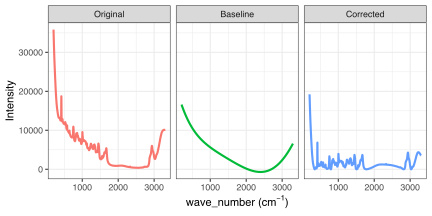
\includegraphics[width=0.8\textwidth,height=\textheight]{figures/fig-profile-baseline-poly-1.pdf}

}

\caption{\label{fig-profile-baseline-poly}The distribution standard
deviation of intensity measurements across wavenumbers.}

\end{figure}

Another source of noise for these data is apparent in the variation of
the intensity measurements across wavelengths within a spectrum. This is
illustrated by the jagged profile illustrated in the ``Original'' and
``Corrected'' panels of Figure~\ref{fig-profile-baseline-poly}.
Smoothing splines and moving averages are two commonly used tools for
reducing this type of noise. The moving average is computed at each
point by averaging a specified number of values about that point. For
example, the moving average of size 10 would replace each point with the
average of the ten points before and after the selected point. The
original curve becomes smoother as the number of points averaged
together becomes larger. Therefore, we must be careful with the number
of points chosen for the smoothing process. Too few points may not
remove enough noise, while too many may remove important signals.

The Savitzky-Golay (SG) procedure (Savitzky and Golay 1964; Stevens and
Ramirez-Lopez 2022) is designed to remove spurious signals by
simultaneously smoothing the data while also centering the overall
signal and dampening variability. The procedure is governed by the order
of differentiation, degree of polynomial, and window size.
Figure~\ref{fig-sg-filtering} compares the impact of this procedure for
differentiation order of 1 or 2, polynomial order of 2, and a small (15)
or large (49) window size. We'll use the notation ``(d, p, w)'' to
describe specifics of SG where the differentiation order, polynomial
order, and window size values are used within the parentheses, such as
(1, 2, 45).

\begin{figure}[t!]

{\centering \includegraphics[width=0.6\textwidth,height=\textheight]{figures/fig-sg-filtering-1.pdf}

}

\caption{\label{fig-sg-filtering}The impact of the Savitzky-Golay
procedure on the Raman spectra.}

\end{figure}

Figure~\ref{fig-lagged-spectra-across-sets} displays the correlation
across the first 1000 wavenumbers for the original data as well as each
of the selected Savitzky-Golay transformations. The effect of
differentiation and window size on the correlation across the
transformed intensities is clear. When comparing first-order
differentiation to second-order differentiation, second-order
differentiation more rapidly reduces correlation among close wavenumbers
up to about the nearest 100 wavenumbers. Increasing the smoothing window
also helps smooth the correlation profiles but does not further reduce
correlation. We will examine the impact of each of these different
smoothing parameter selections on the model performance in the following
sections.

\begin{figure}[t!]

{\centering 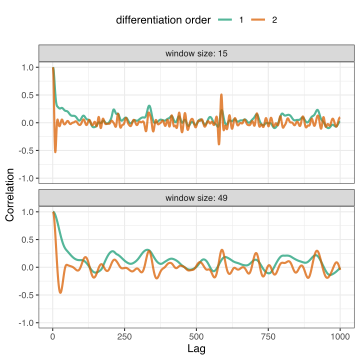
\includegraphics[width=0.7\textwidth,height=\textheight]{figures/fig-lagged-spectra-across-sets-1.pdf}

}

\caption{\label{fig-lagged-spectra-across-sets}The impact of the
Savitzky-Golay procedure on the correlation between lagged wavenumbers.}

\end{figure}

For these data, principal component analysis can be conducted on the
training set predictors (after centering and scaling the predictors).
This can help us understand if there are any unwanted systematic effects
in the data (such as differences in reagents, instruments, etc.).
Figure~\ref{fig-pca-plot} shows the results using two components. These
components accounted for between 65\%-95\% of the predictor information,
with the exception of the (2, 2, 15) set, which only captured about
45\%. With the exception of a single sample, there are no obvious
patterns in the results to give us pause (such as clustering). That odd
sample, number 34, is the same data point in
Figure~\ref{fig-raman-spectra} with relatively low intensity compared to
the other spectra. It is unclear how this would affect the results (if
at all), so it was retained in the data set. Later analyses will examine
whether this sample is associated with larger residuals.

\begin{figure}[t!]

{\centering 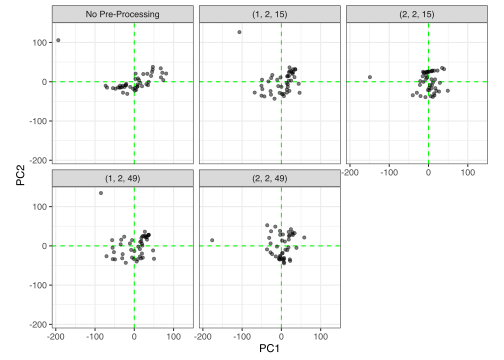
\includegraphics[width=0.8\textwidth,height=\textheight]{figures/fig-pca-plot-1.pdf}

}

\caption{\label{fig-pca-plot}Two-component PCA plots for each
pre-processing method. One particular sample (\#34) has extreme values
for the first principal compoent across all pre-processing methods.}

\end{figure}

\hypertarget{sec-modeling}{%
\section{Machine Learning Models}\label{sec-modeling}}

Over the past half-century, the number and types of models for relating
a set of predictors to a response has rapidly grown. Improvements in
computational power and mathematical complexity have been the primary
drivers of this increase. Traditionally, model complexity is generally
tied to the number of parameters of a model. As the number of model
parameters increases, so does the ability of a model to adapt and morph
to the relationship between predictors and the response. For example,
the basic partial least squares model has one tuning parameter and is
effective at finding a linear relationship between predictors and the
response. However, this method is ineffective at finding non-linear
relationships. In contrast, consider a simple single-layer, feed-forward
neural network. This model can easily have many more parameters than the
number of predictors. For the example data, the number of predictors
already exceeds the number of samples. Therefore, even the simplest of
neural network models can over-fit the available data without
appropriate precautions.

\begin{tcolorbox}[enhanced jigsaw, title=\textcolor{quarto-callout-important-color}{\faExclamation}\hspace{0.5em}{\textbf{WTF} \#9}, rightrule=.15mm, leftrule=.75mm, bottomtitle=1mm, opacityback=0, opacitybacktitle=0.6, bottomrule=.15mm, arc=.35mm, colframe=quarto-callout-important-color-frame, breakable, toprule=.15mm, toptitle=1mm, colback=white, titlerule=0mm, coltitle=black, left=2mm, colbacktitle=quarto-callout-important-color!10!white]

Most ML models (or pre-processors) have tuning parameters: important
parameters that cannot be directly estimated from the data (e.g., unlike
a regression slope).

These parameters usually govern how complex a model can become. Hence,
choosing appropriate tuning parameter values is a pivotal operation
since it controls if the model over- or under-fits the data.

\end{tcolorbox}

As part of the modeling process, we need to find a set of values for the
tuning parameters of each model that effectively uncovers an optimal
predictor-response relationship. As mentioned in the section on data
splitting, the search for an optimal model must be done in the context
of cross-validation to protect the model-building process from
over-fitting to the available data. The next question we must address is
what values of the tuning parameters should be evaluated. A brute-force
approach would be to evaluate many different tuning parameter values and
select the optimal one. More sophisticated techniques are also available
that utilize gradient descent, genetic algorithms, or principles of
experimental design to find an optimal set of parameter values more
efficiently (Ali et al. 2023; Ippolito 2022).

How should the parameter sets be evaluated? Answering this question
depends on the response. When the response is continuous, then the two
most common performance metrics are \(R^2\) and root mean square error
(RMSE) (Neter et al. 1996). Many more options are available when the
response is categorical, and the user must be keenly aware of response
characteristics when selecting the performance metric. For example, if a
categorical outcome is highly imbalanced, then selecting accuracy as the
metric is not advisable. Specifically, it is possible to get high
accuracy simply by classifying all samples into the majority class.
Instead, a metric like the Kappa statistic (Cohen 1960) or area under
the receiver operating characteristic curve (Nahm 2022) may be better
choices for a performance metric since these measurements force a model
to predict the minority class more accurately.

In this manufacturing example, the response is continuous, and the
metric of RMSE will be used to assess predictive performance.

\begin{tcolorbox}[enhanced jigsaw, title=\textcolor{quarto-callout-important-color}{\faExclamation}\hspace{0.5em}{\textbf{WTF} \#10}, rightrule=.15mm, leftrule=.75mm, bottomtitle=1mm, opacityback=0, opacitybacktitle=0.6, bottomrule=.15mm, arc=.35mm, colframe=quarto-callout-important-color-frame, breakable, toprule=.15mm, toptitle=1mm, colback=white, titlerule=0mm, coltitle=black, left=2mm, colbacktitle=quarto-callout-important-color!10!white]

The performance metric that you choose is important; poor choices can
guide you to a ``correct'' answer that might be inappropriate.

For example, \(R^2\) is a measure of correlation but not accuracy.
Optimizing it can yield models that are inaccurate at the high and low
regions of the outcome distribution.

\end{tcolorbox}

While there are many models to choose from, we will compare four
modeling techniques for this data: partial least squares (PLS), random
forest (RF), Cubist, and support vector machines (SVM). These models
were selected to illustrate a range of types of models. We will now
provide a high-level explanation of each of these models along with
additional references.

\hypertarget{partial-least-squares}{%
\subsubsection{Partial Least Squares}\label{partial-least-squares}}

Spectroscopy data has traditionally been modeled using PLS (Htet et al.
2021; Esmonde-White et al. 2017). PLS is a logical technique to use for
this type of data because it naturally handles highly correlated
predictors. This model seeks to find linear combinations of the original
predictors that have an optimal correlation with the response by using
as few linear combinations as possible (Wold, Sjöström, and Eriksson
2001). Specifically, PLS finds linear combinations that summarize
variability across the predictors while simultaneously optimizing their
correlation with the response. The primary tuning parameter for PLS is
the number of linear combinations, or latent variables, to retain.

\hypertarget{random-forest}{%
\subsubsection{Random forest}\label{random-forest}}

Random forest is a recursive partitioning that is built on an ensemble
of trees (Breiman 2001; Seifert 2020). A single tree is constructed by
recursively splitting the data into subsets with greater purity in the
response. The RF model provides an improvement over a single tree by
reducing variance through an ensemble of trees. Specifically, an RF
model does the following process many times: selects a bootstrap sample
of the data and builds a tree on the bootstrap sample. A randomly
selected number of predictors is chosen at each split to construct each
tree. An optimal predictor within the sample is selected, and the
routine proceeds to the next split. Prediction for a new sample is the
average value across the entire ensemble of trees. RF has two primary
tuning parameters: the number of data points within a tree node required
to split the data further and the number of randomly selected predictors
for each split (usually referred to as \(m_{try}\)).

\hypertarget{cubist}{%
\subsubsection{Cubist}\label{cubist}}

The Cubist model is also constructed from an initial ensemble of trees
but in a very different, more complex way than RF (Quinlan 1987). It
uses a model tree rather than a partitioning tree as its foundation. The
primary difference between a partitioning tree and a model tree is that
a model tree constructs a linear model in each terminal node. The paths
through the trees to the terminal node are \emph{rules}, and these rules
are further pruned and/or simplified.

Cubist creates an ensemble of individual rule-based models in a manner
that is similar, but not the same as, boosting (Kuhn and Johnson 2013).
Once the ensemble has been completed, predictions from the samples'
closest neighbors in the training set can further adjust the model
predictions (Quinlan 1993). Cubist has two tuning parameters: the number
of committees and the number of nearest neighbors.

\hypertarget{support-vector-machines}{%
\subsubsection{Support vector machines}\label{support-vector-machines}}

Support vector machines are a modeling technique that uncovers the
relationship between the predictors and the response using samples that
lie outside of a conceptual margin (a boundary about the optimal
relationship) (Drucker et al. 1996; Ullah et al. 2018). Several
nonlinear versions of SVMs exist; the one implemented in this analysis
uses a radial basis function (RBF). For the radial-basis SVM, the number
of samples allowed to be outside of the margin is controlled by the cost
parameter, and the RBF dispersion parameter controls the surface's
flexibility. Therefore, the radial basis SVM has the flexibility to
identify a non-linear relationship between the predictors and the
response.

SVMs are the most difficult to tune out of the four models described
here. The two tuning parameters tend to exhibit traditional interaction
effects so that there can be a small region of good performance within a
larger area of unsuitable models; see, for example,
\href{https://www.tmwr.org/iterative-search\#svm}{Section 14.1} of Kuhn
and Silge (2022).

\hypertarget{modeling-strategy}{%
\section{Modeling Strategy}\label{modeling-strategy}}

For each model, a set of 25 tuning parameter combinations are evaluated.
For PLS and random forest, we'll only tune a single parameter (the
number of PLS components and \(m_{try}\), respectively). For support
vector and Cubist models, a space-filling design (Joseph 2016) is used
to create two-dimensional grids of the parameter space for each model.
These grids are created using Latin hypercube designs that fill the
rectangular parameter space. They often use an additional criterion to
reduce the chances that any of the tuning parameter combinations are too
close (i.e., redundant). The \emph{modeling process} has 3-4 parameters:
1-2 from the models themselves and two from the pre-processing (i.e.,
differentiation order and the smoothing window size).

For each tuning parameter combination, 5 repeats of 10-fold
cross-validation are used to appropriately estimate the RMSE for future
samples. We will examine the relationship between the tuning parameters
and the estimated RMSE to help understand the performance patterns and
to choose reasonable values for the parameters.

\begin{tcolorbox}[enhanced jigsaw, title=\textcolor{quarto-callout-important-color}{\faExclamation}\hspace{0.5em}{\textbf{WTF} \#11}, rightrule=.15mm, leftrule=.75mm, bottomtitle=1mm, opacityback=0, opacitybacktitle=0.6, bottomrule=.15mm, arc=.35mm, colframe=quarto-callout-important-color-frame, breakable, toprule=.15mm, toptitle=1mm, colback=white, titlerule=0mm, coltitle=black, left=2mm, colbacktitle=quarto-callout-important-color!10!white]

Despite the literature, optimizing hyper-parameters using grid search is
effective and can be very efficient using advanced (but easy to use)
computational and statistical methods

\end{tcolorbox}

One computational tool for speeding up grid search is parallel
processing. None of the 1,250 models estimated in the grid search depend
on any other and, as such, can be executed simultaneously on different
computer CPU cores. Software can seamlessly facilitate this, and it is
not uncommon to see at least 5-fold reductions in the computational time
using this method (Kuhn and Silge 2022).

Also, there are statistical methods to evaluate 25 models without having
to estimate all of them. For example, for some models, the most complex
model can be fit, and results from sub-models can be derived at no extra
cost. For example, if a Cubist model is created with an ensemble size of
50, we can get predictions from the same model for sizes 1 - 49 at
negligible computational cost. Additionally, racing methods (Kuhn 2014)
can conduct interim analyses during grid search and remove tuning
parameter combinations that are unlikely to be chosen as the best
results. This can enable users to screen a large number of models and
pre-processing methods quickly.

Finally, grid search had been considered inefficient because of the
assumption that regular (i.e., full factorial) grids were used. If we
evaluated \(L\) values of each of \(M\) tuning parameters, the full
factorial set of \(L^M\) combinations can become very large. This is no
surprise to most CMC statisticians and engineers. However, as previously
mentioned, the better design choices for grid search are space-filling
designs. It is difficult to quantify the positive impact these designs
have had on optimizing models in terms of efficiency and efficacy.
Figure~\ref{fig-sfd} shows an example Audze-Eglais design from Husslage
et al. (2011) for the two Cubist tuning parameters and 25 candidate
points.

\begin{figure}[t!]

{\centering \includegraphics[width=0.45\textwidth,height=\textheight]{figures/fig-sfd-1.pdf}

}

\caption{\label{fig-sfd}An example of a space-filling design for two
tuning parameters in a Cubist model.}

\end{figure}

An alternate tool called Bayesian optimization (Gramacy 2020) was used
to optimize the support vector machine models. It starts with a small
grid of results, in our case, a space-filling design with ten tuning
parameter combinations. These initial results are used as substrate for
a Gaussian Process (GP) model (Rasmussen, Williams, et al. 2006) where
the resampled RMSE values are the outcomes, and the SVM tuning
parameters (cost and RBF dispersion) are the predictors. The GP then
predicts the next tuning parameter combination to resample. Once those
results are available, the process repeats. Fifteen iterations of this
iterative optimization process were used to evaluate a total of 25
tuning parameter combinations for the SVM models.

\hypertarget{model-tuning-results}{%
\section{Model Tuning Results}\label{model-tuning-results}}

First, let's examine the PLS and RF model results, each of which
optimized a single tuning parameter.
Figure~\ref{fig-pls-rf-tune-profiles} (left) illustrates the
relationship between the number of PLS components and the RMSE. There
are separate profiles for the different Savitzky-Golay configurations.
RMSE generally decreases as the number of components increases
regardless of whether or not the spectra were pre-processed. Oddly, the
(1, 2, 49) configuration showed degradation in performance after 8
components. The model with the lowest RMSE uses the (1, 2, 15)
pre-processor and 12 components. There was a plateau of RMSE after 12
components but choosing fewer components is better than adding
unnecessary complexity.

\begin{figure}[t!]

{\centering 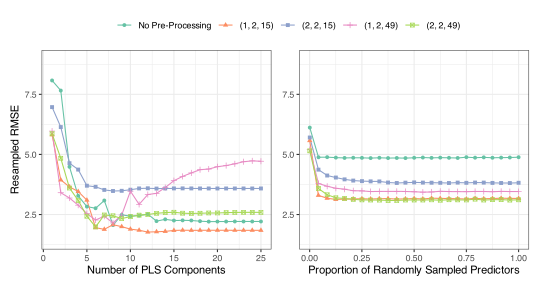
\includegraphics[width=0.9\textwidth,height=\textheight]{figures/fig-pls-rf-tune-profiles-1.pdf}

}

\caption{\label{fig-pls-rf-tune-profiles}The tuning parameter profiles
for partial least squares and random forest.}

\end{figure}

Figure~\ref{fig-pls-rf-tune-profiles} (right) displays the tuning
parameter profile for the RF model. Since the different pre-processing
methods can produce different numbers of predictors, \(m_{try}\) is
represented here as a proportion of the number of possible predictors.
The value of \(m_{try}\) is fairly irrelevant so long as at least 10\%
of the predictors are randomly sampled at each split. The numerically
best random forest model used 1,273 predictors with pre-processing
strategy (2, 2, 49), although there is obviously a range of values with
the same performance (as well as another pre-processor). The optimal RF
model (with RMSE 3.08) performs poorly compared to the optimal PLS model
(RMSE = 1.77).

The Cubist performance profiles are shown in
Figure~\ref{fig-cb-profiles}. The left panel shows that, after a few
initial iterations, choice of the ensemble size is not crucial On the
right, the main trend in the number of nearest neighbors is that 1-2
neighbors is a poor choice; otherwise there is very little difference in
the RMSE profiles. Across pre-processing configurations, the (2, 2, 49)
SG configuration, along with 9 committees and 7 neighbors, appears to
work best with this model with an estimated RMSE of 1.79. Like the
random forest results, pre-processing has a larger impact than the
model's tuning parameter(s).

\begin{figure}[t!]

{\centering 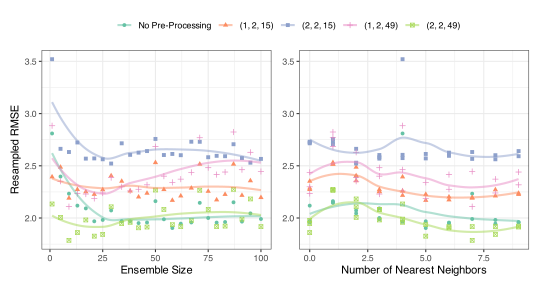
\includegraphics[width=0.9\textwidth,height=\textheight]{figures/fig-cb-profiles-1.pdf}

}

\caption{\label{fig-cb-profiles}The tuning parameter profiles for the
Cubist model.}

\end{figure}

Recall that SVM models the parameter space; there are sometimes isolated
regions of good performance. An initial grid of 10 tuning parameter
candidates were selected before proceeding to the iterative
calculations. Across all pre-processing methods, the best RMSE from the
initial phase was 4.91, a substandard result.

Figure~\ref{fig-svm-search} illustrates the process of the iterative
Bayesian search. A few of the profiles show a progressive reduction in
the RMSE as the algorithm moves through the parameter space defined by
the SVM cost and RBF dispersion parameters. Other profiles show some
sporadic increases/jumps in RMSE. Bayesian optimization is a global,
derivative free technique and may make discordant jumps as it explores
the parameter space. In the end, the average reduction in RMSE across
the pre-processing settings was 3.1-fold, indicating that the
optimization was effective. There are a few pre-processing methods with
effectively equal results. The numerically best corresponding to SG
settings of (2, 2, 49), a cost value of 29.7, and a radial basis
function dispersion parameter of 0.0000445 The corresponding RMSE was
estimated to be 1.8.

\begin{figure}[t!]

{\centering 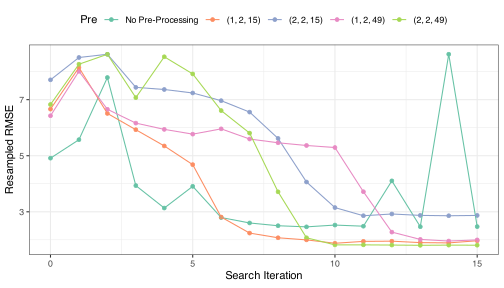
\includegraphics[width=0.9\textwidth,height=\textheight]{figures/fig-svm-search-1.pdf}

}

\caption{\label{fig-svm-search}Progress of Bayesian optimization for the
SVM parameters. Iteration zero reflects the best candidate value from
the initial grid search.}

\end{figure}

There are a few significant trends in these results. First, random
forest, with these particular pre-processing methods, was uniformly the
worst model. In terms of pre-processing:

\begin{itemize}
\item
  The (2, 2, 15) SG configuration was also particularly ineffective
  across models.
\item
  The other pre-processed versions of the data had decent, if not fine,
  results.
\item
  No pre-processing, in some cases, could work well with these models
  and this data.
\end{itemize}

Given the confidence intervals on the best RMSE, multiple pre-processing
choices have equal performance.

\begin{figure}[t!]

{\centering 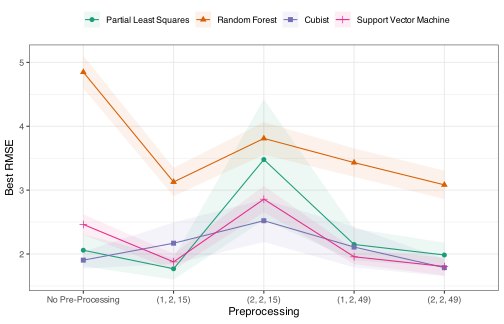
\includegraphics[width=0.75\textwidth,height=\textheight]{figures/fig-all-optimal-models-1.pdf}

}

\caption{\label{fig-all-optimal-models}Cross-validation predictive
performance using the optimal tuning parameter settings for each
predictor set and model. The colored regions are approximate 90\%
confidence intervals.}

\end{figure}

\begin{tcolorbox}[enhanced jigsaw, title=\textcolor{quarto-callout-important-color}{\faExclamation}\hspace{0.5em}{\textbf{WTF} \#12}, rightrule=.15mm, leftrule=.75mm, bottomtitle=1mm, opacityback=0, opacitybacktitle=0.6, bottomrule=.15mm, arc=.35mm, colframe=quarto-callout-important-color-frame, breakable, toprule=.15mm, toptitle=1mm, colback=white, titlerule=0mm, coltitle=black, left=2mm, colbacktitle=quarto-callout-important-color!10!white]

It is a common situation when multiple tuning parameter combinations
have approximately the same level of performance within and between
models. Likewise, it is rare that a single type of model completely
outclasses the others.

\end{tcolorbox}

Let's compare the observed versus predicted values across the five
pre-processing sets and three models.
Figure~\ref{fig-obs-pred-cv-comparison} highlights some interesting
characteristics. First, there is one sample that tends to have very
large residuals. This is our old friend sample 34, last seen in
Figure~\ref{fig-pca-plot}. Interestingly, some models are more sensitive
to this sample than others. The SVM model is remarkably robust to the
sample. It may be because of the nature of support vector machines: they
do not use all of the training set data to define the prediction
equation. It is possible that sample 34 is not one of the \emph{support
vectors} for this model.

At this point, the sample is very interesting, and we would consult with
the spectroscopist to determine if it is valid. That could be an issue
with reagents or instrumentation. For our analysis here, we'll leave it
alone and pick a model/pre-processing combination that appears
unaffected.

\begin{figure}[t!]

{\centering 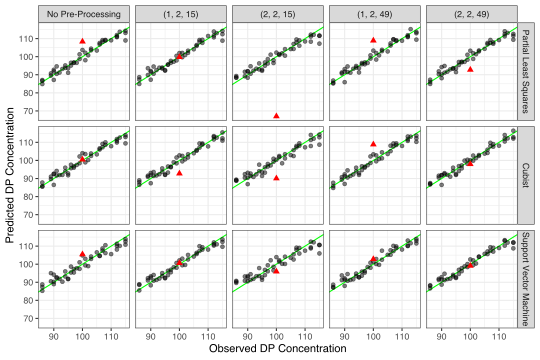
\includegraphics[width=0.9\textwidth,height=\textheight]{figures/fig-obs-pred-cv-comparison-1.pdf}

}

\caption{\label{fig-obs-pred-cv-comparison}Comparison of observed versus
hold-out predicted values from cross-validation for the optimal tuning
parameter settings for three models. One challenging sample to predict
is highlighted in red.}

\end{figure}

We must pick a pre-processing scheme and model type to define the
official model. We'll choose the PLS model with 12 components and the
(1, 2, 15) pre-processing settings. The performance of this model is
exceptional, especially given that a linear model has limited complexity
(generally, simpler is better). The final model fit uses the optimized
tuning parameters in conjunction with the entire training set of 45
samples.

Now that we have the official model fit, our next step is to verify the
results using the test set.

As an alternative to choosing between models, a \emph{stacking ensemble}
could selectively blend all of our existing models (and pre-processing
methods) into a single model fit. These models can dynamically choose
which methods to include or exclude to maximize performance (Breiman
1996; Smyth and Wolpert 1999).

\begin{tcolorbox}[enhanced jigsaw, title=\textcolor{quarto-callout-important-color}{\faExclamation}\hspace{0.5em}{\textbf{WTF} \#13}, rightrule=.15mm, leftrule=.75mm, bottomtitle=1mm, opacityback=0, opacitybacktitle=0.6, bottomrule=.15mm, arc=.35mm, colframe=quarto-callout-important-color-frame, breakable, toprule=.15mm, toptitle=1mm, colback=white, titlerule=0mm, coltitle=black, left=2mm, colbacktitle=quarto-callout-important-color!10!white]

Stacking is worth trying if the training set is large. In these
situations, it typically yields ensembles with slightly better results.
Its importance has been inflated due to success in machine learning
competitions.

\end{tcolorbox}

\hypertarget{test-set-results}{%
\section{Test Set Results}\label{test-set-results}}

Figure~\ref{fig-test} shows the observed and predicted drug product
concentrations for the 15 samples in the test set. The sample size is
small, but there does appear to be some excess variation in the
predictors for smaller values. Despite this, the results seem reasonably
good.

The resulting test set RMSE was 1.93 (compared to the resampling
estimate of 1.77). The corresponding test set \(R^2\) was 95.8\%.

\begin{figure}[t!]

{\centering 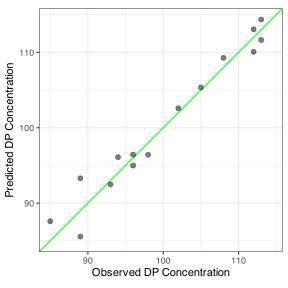
\includegraphics[width=0.5\textwidth,height=\textheight]{figures/fig-test-1.pdf}

}

\caption{\label{fig-test}Observed and predicted values for the test
set.}

\end{figure}

\hypertarget{post-modeling-activities}{%
\section{Post-Modeling Activities}\label{post-modeling-activities}}

Assuming our final model will be used on additional unknown samples in
the future, there are a few more tasks. First is documentation. This
should involve descriptions of the training and test sets, their
provenance, the process of optimizing and choosing the final model, and
a description of its use case.

The amount of documentation and what should be included depends on how
the predictions will be used and by whom. Speaking from experience
regarding models for ADMET endpoints, the consumers of the model
predictions were very focused on results for yet-to-be-synthesized
molecules. Inconsistencies in predictions (real or perceived) could lead
to intense interest in the model's particulars. Good documentation about
what the model was good for (and not suitable for) was critical.
\emph{Model Cards} (Mitchell et al. 2019) offer a good template for
getting started.

\begin{tcolorbox}[enhanced jigsaw, title=\textcolor{quarto-callout-important-color}{\faExclamation}\hspace{0.5em}{\textbf{WTF} \#14}, rightrule=.15mm, leftrule=.75mm, bottomtitle=1mm, opacityback=0, opacitybacktitle=0.6, bottomrule=.15mm, arc=.35mm, colframe=quarto-callout-important-color-frame, breakable, toprule=.15mm, toptitle=1mm, colback=white, titlerule=0mm, coltitle=black, left=2mm, colbacktitle=quarto-callout-important-color!10!white]

Defining and documenting the model's intended use is essential and is
called its applicability. If a wide variety of people can access the
model, it is hard to control who will use it and for what purpose.
Setting intentional limits of relevance is a good idea.

\end{tcolorbox}

In some cases, explaining how the model works and why it made specific
predictions is necessary. Unfortunately, these questions may be asked if
a prediction fails to meet preconceived expectations. Simpler models,
such as PLS, are easier to explain. Regardless of model complexity,
there is a rich field of research on model explainers. See, for example,
Molnar (2020) and Biecek and Burzykowski (2021) for tools to help users
understand the model and its results. Finally, if a model is put into
production, we must ensure it still meets its stated goals (i.e.,
applicability). If more labeled samples are being accrued, a protocol
for monitoring performance over time is critical in case the performance
statistics begin to drift away from their original resampling/test set
estimates.

\begin{tcolorbox}[enhanced jigsaw, title=\textcolor{quarto-callout-important-color}{\faExclamation}\hspace{0.5em}{\textbf{WTF} \#15}, rightrule=.15mm, leftrule=.75mm, bottomtitle=1mm, opacityback=0, opacitybacktitle=0.6, bottomrule=.15mm, arc=.35mm, colframe=quarto-callout-important-color-frame, breakable, toprule=.15mm, toptitle=1mm, colback=white, titlerule=0mm, coltitle=black, left=2mm, colbacktitle=quarto-callout-important-color!10!white]

\emph{Models} do not drift; data can change over time, as can the
population being predicted. Tools called applicability domain methods
(Netzeva et al. 2005; Gadaleta et al. 2016) help measure how far (if at
all) a new sample is from the original training set (i.e.,
extrapolation). These values can accompany a new sample prediction to
help gauge how dodgy a new sample may be.

\end{tcolorbox}

The nature of drug discovery causes the type, structure, and
characteristics of molecules to change over time; medicinal chemists are
designing therapies entirely different from those created in decades
past. Physiochemical properties fluctuate over time; knowing how the
model handles these changes is vital.

There is also the idea of \emph{concept drift}: the purpose of a model
can also change. For example, suppose that we develop an ADMET ML model
for predicting blood-brain barrier permeation based on existing
therapeutic areas. Suppose the company purchases other discovery groups
with a strong neuroscience group (where there was none). The original
model was intended to tell when a molecule unintentionally crossed the
barrier. Now, there is increased interest in molecules that should cross
the barrier. At this point, an assessment should be made as to whether a
separate model is required for each use case.

\hypertarget{conclusions}{%
\section{Conclusions}\label{conclusions}}

This tutorial was intended to provide readers with a realistic worked
example of machine learning with a CMC application and demonstrate that
there is still a fair amount of art in this particular area of science.
The content in most of our WTF items is borne out of experience. Our
advice for practitioners starting out is to read as much literature as
possible, try many different approaches, and be very dogmatic about
thoroughly validating your results.

\hypertarget{software-and-data}{%
\section{Software and Data}\label{software-and-data}}

The code and data used to create this tutorial are found on
GitHub\footnote{\href{https://github.com/kjell-stattenacity/Tutorial}{\texttt{https://github.com/kjell-stattenacity/Tutorial}}}.
\href{http://cran.r-project.org}{R version 4.2.2 (2022-10-31)} was used
to create the analyses, and \href{https://quarto.org}{Quarto version
1.3.450} was used to create the pre-print document and website. The
GitHub repository lists specific R package versions that were used.

\hypertarget{references}{%
\section*{References}\label{references}}
\addcontentsline{toc}{section}{References}

\hypertarget{refs}{}
\begin{CSLReferences}{1}{0}
\leavevmode\vadjust pre{\hypertarget{ref-Abdi2010p3532}{}}%
Abdi, Herve, and Lynne Williams. 2010. {``Principal Component
Analysis.''} \emph{Wiley Interdisciplinary Reviews: Computational
Statistics} 2 (4): 433--59.

\leavevmode\vadjust pre{\hypertarget{ref-ali2023hyperparameter}{}}%
Ali, Yasser A, Emad Mahrous Awwad, Muna Al-Razgan, and Ali Maarouf.
2023. {``Hyperparameter Search for Machine Learning Algorithms for
Optimizing the Computational Complexity.''} \emph{Processes} 11 (2):
349.

\leavevmode\vadjust pre{\hypertarget{ref-biecek2021explanatory}{}}%
Biecek, Przemyslaw, and Tomasz Burzykowski. 2021. \emph{Explanatory
Model Analysis: Explore, Explain, and Examine Predictive Models}. CRC
Press.

\leavevmode\vadjust pre{\hypertarget{ref-Borisov2022}{}}%
Borisov, Vadim, Tobias Leemann, Kathrin Sessler, Johannes Haug, Martin
Pawelczyk, and Gjergji Kasneci. 2022. {``Deep Neural Networks and
Tabular Data: A Survey.''} \emph{{IEEE} Transactions on Neural Networks
and Learning Systems}, 1--21.

\leavevmode\vadjust pre{\hypertarget{ref-breiman1996stacked}{}}%
Breiman, Leo. 1996. {``Stacked Regressions.''} \emph{Machine Learning}
24: 49--64.

\leavevmode\vadjust pre{\hypertarget{ref-breiman2001random}{}}%
---------. 2001. {``Random Forests.''} \emph{Machine Learning} 45:
5--32.

\leavevmode\vadjust pre{\hypertarget{ref-charu2018neural}{}}%
Charu, Aggarwal. 2018. \emph{Neural Networks and Deep Learning: A
Textbook}. Spinger.

\leavevmode\vadjust pre{\hypertarget{ref-cleveland1988locally}{}}%
Cleveland, William S, and Susan J Devlin. 1988. {``Locally Weighted
Regression: An Approach to Regression Analysis by Local Fitting.''}
\emph{Journal of the American Statistical Association} 83 (403):
596--610.

\leavevmode\vadjust pre{\hypertarget{ref-cohen1960coefficient}{}}%
Cohen, Jacob. 1960. {``A Coefficient of Agreement for Nominal Scales.''}
\emph{Educational and Psychological Measurement} 20 (1): 37--46.

\leavevmode\vadjust pre{\hypertarget{ref-drucker1996support}{}}%
Drucker, Harris, Christopher J Burges, Linda Kaufman, Alex Smola, and
Vladimir Vapnik. 1996. {``Support Vector Regression Machines.''}
\emph{Advances in Neural Information Processing Systems} 9.

\leavevmode\vadjust pre{\hypertarget{ref-esmonde2022role}{}}%
Esmonde-White, Karen A, Maryann Cuellar, and Ian R Lewis. 2022. {``The
Role of Raman Spectroscopy in Biopharmaceuticals from Development to
Manufacturing.''} \emph{Analytical and Bioanalytical Chemistry}, 1--23.

\leavevmode\vadjust pre{\hypertarget{ref-esmonde2017raman}{}}%
Esmonde-White, Karen A, Maryann Cuellar, Carsten Uerpmann, Bruno Lenain,
and Ian R Lewis. 2017. {``Raman Spectroscopy as a Process Analytical
Technology for Pharmaceutical Manufacturing and Bioprocessing.''}
\emph{Analytical and Bioanalytical Chemistry} 409 (3): 637--49.

\leavevmode\vadjust pre{\hypertarget{ref-gadaleta2016applicability}{}}%
Gadaleta, Domenico, Giuseppe Felice Mangiatordi, Marco Catto, Angelo
Carotti, and Orazio Nicolotti. 2016. {``Applicability Domain for QSAR
Models: Where Theory Meets Reality.''} \emph{International Journal of
Quantitative Structure-Property Relationships (IJQSPR)} 1 (1): 45--63.

\leavevmode\vadjust pre{\hypertarget{ref-goodfellow2016deep}{}}%
Goodfellow, Ian, Yoshua Bengio, and Aaron Courville. 2016. \emph{Deep
Learning}. MIT press.

\leavevmode\vadjust pre{\hypertarget{ref-gorishniy2021revisiting}{}}%
Gorishniy, Yury, Ivan Rubachev, Valentin Khrulkov, and Artem Babenko.
2021. {``Revisiting Deep Learning Models for Tabular Data.''}
\emph{Advances in Neural Information Processing Systems} 34: 18932--43.

\leavevmode\vadjust pre{\hypertarget{ref-gramacy2020surrogates}{}}%
Gramacy, Robert B. 2020. \emph{Surrogates: Gaussian Process Modeling,
Design, and Optimization for the Applied Sciences}. CRC press.

\leavevmode\vadjust pre{\hypertarget{ref-hasan2021missing}{}}%
Hasan, Md Kamrul, Md Ashraful Alam, Shidhartho Roy, Aishwariya Dutta, Md
Tasnim Jawad, and Sunanda Das. 2021. {``Missing Value Imputation Affects
the Performance of Machine Learning: A Review and Analysis of the
Literature (2010--2021).''} \emph{Informatics in Medicine Unlocked} 27:
100799.

\leavevmode\vadjust pre{\hypertarget{ref-HastieEtAl2017}{}}%
Hastie, T, R Tibshirani, and J Friedman. 2017. \emph{{The Elements of
Statistical Learning: Data Mining, Inference and Prediction}}. Springer.

\leavevmode\vadjust pre{\hypertarget{ref-Hawkins2004p1}{}}%
Hawkins, D. 2004. {``The Problem of Overfitting.''} \emph{Journal of
Chemical Information and Computer Sciences} 44 (1): 1--12.

\leavevmode\vadjust pre{\hypertarget{ref-hoerl1970ridge}{}}%
Hoerl, Arthur E, and Robert W Kennard. 1970. {``Ridge Regression: Biased
Estimation for Nonorthogonal Problems.''} \emph{Technometrics} 12 (1):
55--67.

\leavevmode\vadjust pre{\hypertarget{ref-htet2021pls}{}}%
Htet, Tar Tar Moe, Jordi Cruz, Putthiporn Khongkaew, Chaweewan
Suwanvecho, Leena Suntornsuk, Nantana Nuchtavorn, Waree Limwikrant, and
Chutima Phechkrajang. 2021. {``PLS-Regression-Model-Assisted Raman
Spectroscopy for Vegetable Oil Classification and Non-Destructive
Analysis of Alpha-Tocopherol Contents of Vegetable Oils.''}
\emph{Journal of Food Composition and Analysis} 103: 104119.

\leavevmode\vadjust pre{\hypertarget{ref-husslage2011space}{}}%
Husslage, Bart GM, Gijs Rennen, Edwin R Van Dam, and Dick Den Hertog.
2011. {``Space-Filling Latin Hypercube Designs for Computer
Experiments.''} \emph{Optimization and Engineering} 12: 611--30.

\leavevmode\vadjust pre{\hypertarget{ref-ippolito2022hyperparameter}{}}%
Ippolito, Pier Paolo. 2022. {``Hyperparameter Tuning: The Art of
Fine-Tuning Machine and Deep Learning Models to Improve Metric
Results.''} In \emph{Applied Data Science in Tourism: Interdisciplinary
Approaches, Methodologies, and Applications}, 231--51. Springer.

\leavevmode\vadjust pre{\hypertarget{ref-jesus2020raman}{}}%
Jesus, José Izo Santana da Silva de, Raimar Löbenberg, and Nadia Araci
Bou-Chacra. 2020. {``Raman Spectroscopy for Quantitative Analysis in the
Pharmaceutical Industry.''} \emph{Journal of Pharmacy and Pharmaceutical
Sciences} 23 (1): 24--46.

\leavevmode\vadjust pre{\hypertarget{ref-joseph2016space}{}}%
Joseph, V. 2016. {``Space-Filling Designs for Computer Experiments: {A}
Review.''} \emph{Quality Engineering} 28 (1): 28--35.

\leavevmode\vadjust pre{\hypertarget{ref-kadra2021regularization}{}}%
Kadra, Arlind, Marius Lindauer, Frank Hutter, and Josif Grabocka. 2021.
{``Regularization Is All You Need: Simple Neural Nets Can Excel on
Tabular Data.''} \emph{arXiv} 536.

\leavevmode\vadjust pre{\hypertarget{ref-kuhn2014futility}{}}%
Kuhn, Max. 2014. {``Futility Analysis in the Cross-Validation of Machine
Learning Models.''} \emph{arXiv}.

\leavevmode\vadjust pre{\hypertarget{ref-kuhn2013applied}{}}%
Kuhn, Max, and Kjell Johnson. 2013. \emph{Applied Predictive Modeling}.
Springer.

\leavevmode\vadjust pre{\hypertarget{ref-fes}{}}%
---------. 2019. \emph{Feature Engineering and Selection: A Practical
Approach for Predictive Models}. CRC Press.

\leavevmode\vadjust pre{\hypertarget{ref-tmwr}{}}%
Kuhn, Max, and Julia Silge. 2022. \emph{Tidy Modeling with {R}}.
O'Reilly Media, Inc.

\leavevmode\vadjust pre{\hypertarget{ref-luers1971polynomial}{}}%
Luers, James K, and Robert H Wenning. 1971. {``Polynomial
Smoothing---Linear Vs Cubic.''} \emph{Technometrics} 13 (3): 589--600.

\leavevmode\vadjust pre{\hypertarget{ref-Massy1965p234}{}}%
Massy, William. 1965. {``Principal Components Regression in Exploratory
Statistical Research.''} \emph{Journal of the American Statistical
Association} 60: 234--46.

\leavevmode\vadjust pre{\hypertarget{ref-mitchell2019model}{}}%
Mitchell, Margaret, Simone Wu, Andrew Zaldivar, Parker Barnes, Lucy
Vasserman, Ben Hutchinson, Elena Spitzer, Inioluwa Deborah Raji, and
Timnit Gebru. 2019. {``Model Cards for Model Reporting.''} In
\emph{Proceedings of the Conference on Fairness, Accountability, and
Transparency}, 220--29.

\leavevmode\vadjust pre{\hypertarget{ref-molnar2020interpretable}{}}%
Molnar, Christoph. 2020. \emph{Interpretable Machine Learning}.
Independently published.

\leavevmode\vadjust pre{\hypertarget{ref-nahm2022receiver}{}}%
Nahm, Francis Sahngun. 2022. {``Receiver Operating Characteristic Curve:
Overview and Practical Use for Clinicians.''} \emph{Korean Journal of
Anesthesiology} 75 (1): 25--36.

\leavevmode\vadjust pre{\hypertarget{ref-neter1996applied}{}}%
Neter, John, Michael H Kutner, Christopher J Nachtsheim, William
Wasserman, et al. 1996. {``Applied Linear Statistical Models.''}

\leavevmode\vadjust pre{\hypertarget{ref-netzeva2005current}{}}%
Netzeva, Tatiana I, Andrew P Worth, Tom Aldenberg, Romualdo Benigni,
Mark TD Cronin, Paola Gramatica, Joanna S Jaworska, et al. 2005.
{``Current Status of Methods for Defining the Applicability Domain of
(Quantitative) Structure-Activity Relationships.''} \emph{Alternatives
to Laboratory Animals} 33 (2): 155--73.

\leavevmode\vadjust pre{\hypertarget{ref-quinlan1987simplifying}{}}%
Quinlan, J. Ross. 1987. {``Simplifying Decision Trees.''}
\emph{International Journal of Man-Machine Studies} 27 (3): 221--34.

\leavevmode\vadjust pre{\hypertarget{ref-Quinlan1993p1150}{}}%
---------. 1993. {``Combining Instance-Based and Model-Based
Learning.''} \emph{Proceedings of the Tenth International Conference on
Machine Learning}, 236--43.

\leavevmode\vadjust pre{\hypertarget{ref-rasmussen2006gaussian}{}}%
Rasmussen, Carl Edward, Christopher KI Williams, et al. 2006.
\emph{Gaussian Processes for Machine Learning}. Vol. 1. Springer.

\leavevmode\vadjust pre{\hypertarget{ref-rinnan2009review}{}}%
Rinnan, Åsmund, Frans Van Den Berg, and Søren Balling Engelsen. 2009.
{``Review of the Most Common Pre-Processing Techniques for Near-Infrared
Spectra.''} \emph{TrAC Trends in Analytical Chemistry} 28 (10):
1201--22.

\leavevmode\vadjust pre{\hypertarget{ref-savitzky1964smoothing}{}}%
Savitzky, Abraham, and Marcel JE Golay. 1964. {``Smoothing and
Differentiation of Data by Simplified Least Squares Procedures.''}
\emph{Analytical Chemistry} 36 (8): 1627--39.

\leavevmode\vadjust pre{\hypertarget{ref-seifert2020application}{}}%
Seifert, Stephan. 2020. {``Application of Random Forest Based Approaches
to Surface-Enhanced Raman Scattering Data.''} \emph{Scientific Reports}
10 (1): 5436.

\leavevmode\vadjust pre{\hypertarget{ref-SHWARTZZIV202284}{}}%
Shwartz-Ziv, Ravid, and Amitai Armon. 2022. {``Tabular Data: Deep
Learning Is Not All You Need.''} \emph{Information Fusion} 81: 84--90.

\leavevmode\vadjust pre{\hypertarget{ref-silge2022trends}{}}%
Silge, A, Karina Weber, D Cialla-May, L Müller-Bötticher, D Fischer, and
J Popp. 2022. {``Trends in Pharmaceutical Analysis and Quality Control
by Modern Raman Spectroscopic Techniques.''} \emph{TrAC Trends in
Analytical Chemistry} 153: 116623.

\leavevmode\vadjust pre{\hypertarget{ref-smyth1999linearly}{}}%
Smyth, Padhraic, and David Wolpert. 1999. {``Linearly Combining Density
Estimators via Stacking.''} \emph{Machine Learning} 36: 59--83.

\leavevmode\vadjust pre{\hypertarget{ref-stevens2022}{}}%
Stevens, Antoine, and Leornardo Ramirez-Lopez. 2022. \emph{An
Introduction to the Prospectr Package}.

\leavevmode\vadjust pre{\hypertarget{ref-ullah2018raman}{}}%
Ullah, Rahat, Saranjam Khan, Samina Javaid, Hina Ali, Muhammad Bilal,
and Muhammad Saleem. 2018. {``Raman Spectroscopy Combined with a Support
Vector Machine for Differentiating Between Feeding Male and Female
Infants Mother's Milk.''} \emph{Biomedical Optics Express} 9 (2):
844--51.

\leavevmode\vadjust pre{\hypertarget{ref-wold2001pls}{}}%
Wold, Svante, Michael Sjöström, and Lennart Eriksson. 2001.
{``PLS-Regression: A Basic Tool of Chemometrics.''} \emph{Chemometrics
and Intelligent Laboratory Systems} 58 (2): 109--30.

\end{CSLReferences}



\end{document}
